\section{Erfassungsprogramm}
\label{kap:Erfassungsprogramm}
Das Lesen, bzw. Speichern der Sensordaten erfolgt mit einem Programm, welches sich als Client mit dem Server verbindet und �ber WLAN die Daten aller Sensoren empf�ngt. Die Sensorwerte werden nicht automatisch gespeichert, jedoch empfangen und k�nnen grafisch dargestellt werden (x-, y-, z-Werte f�r jeden Sensor in einer �bersicht). Ist das Speichern der Daten gew�nscht, so muss eine Anzahl an Samples angegeben und der Button \textit{Record to db} bet�tigt werden. Das Speichern der Daten erfolgt dann in eine lokale SQL-Datenbank.

\subsection{Beschreibung HMI - Main}
\label{kap:ClientGraphProgramm}
Die HMI gliedert sich in mehrere Bereiche, in denen verschiedene Funktionalit�ten bereitgestellt werden. Diese finden im folgenden Abschnitt Erl�uterung. 

\begin{figure}[H]
\centering
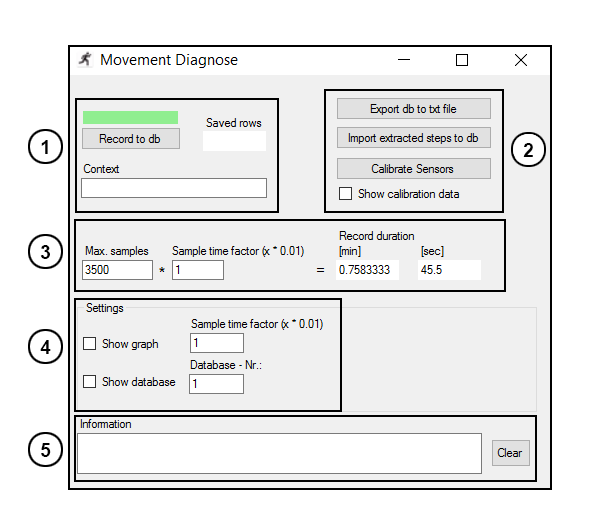
\includegraphics[width=1.0\linewidth]{03_Grafiken/Messsystem/ClientGraph_Gui}
\caption[Client Graph HMI]{Client Graph HMI}
\label{fig:clientgraphgui}
\end{figure}

\begin{enumerate}
	\item \textbf{Aufnahme starten} \\
	Der gr�ne Balken dient als Indikator, ob Messwerte empfangen werden (gr�n: Messung kann gestartet werden, rot: Es werden keine Daten empfangen).\\
	Durch das Bet�tigen des Buttons \textit{Record to db} wird eine Messung gestartet bis diese abgebrochen oder die max. Anzahl an Samples erreicht wird.\\
	Das Label \textit{Saved rows} zeigt die aktuelle Anzahl aufgenommener Messwerte an.\\
	Im Textfeld \textit{Context} kann eine Bezeichnung der Messwerte eingegeben werden (die exportierten Textdateien tragen diesen Namen).
	
	\item \textbf{Import / Export und Kalibrierung}\\
	Mit dem Bet�tigen des Buttons \textit{Export...} erfolgt das Exportieren der erfassten Sensordaten in eine CSV-Datei. Jeder Sensor generiert eine eigene Datei mit dem unter \textit{Context} angegebenen Namen.\\
	Durch das Bet�tigen des Buttons \textit{Import...} kann eine Textdatei (CSV-Format) eingelesen und in die Datenbank geschrieben werden.\\
	Durch das Bet�tigen des Buttons \textit{Calibrate Sensors} erfolgt das Kalibrieren aller Sensoren (s. Beschreibung in \ref{kap:Erfassungsprogramm}). Durch das Setzen des H�kchens \textit{Show...} erfolgt das Darstellen der kalibrierten Sensorwerte.
	
	\item \textbf{Aufnahmezeit}\\
	In das Textfeld \textit{Max. samples} wird die aufzunehmende Anzahl an Messwerten eingetragen. Danach stoppt die Messung automatisch. Standardm��ig sind 3500 Samples eingetragen, da bei einer zu gro�en Anzahl eine \textit{Out of memory Exception} geworfen wird.
	
	\item \textbf{Settings}\\
	Durch das Setzen des H�kchens bei \textit{Show graph} werden die Sensorwerte visualisiert.\\
	Durch das Setzen des H�kchens bei \textit{Show database} werden die Eintr�ge der Datenbank dargestellt.
	
	\item \textbf{Information}\\
	In dem Textfeld erfolgt das Darstellen wichtiger Systemereignisse (z.B. Fehler), die durch das Bet�tigen des Buttons \textit{Clear} gel�scht werden k�nnen.
\end{enumerate}


\subsection{Beschreibung HMI - Visualisierung}
\label{kap:ClientGraphProgrammVisu}
Durch das Bet�tigen des Buttons \textit{Show graph} innerhalb der Hauptansicht des Programms, erfolgt das Darstellen der Visualisierung.\\
Das Visualisieren der Sensorwerte erfolgt durch vier Diagramme pro Sensor (s. Abbildung \ref{fig:clientgraphdiagramm}), in denen die Beschleunigungswerte in jeder Achse einzeln und einmal alle zusammen dargestellt werden. 
Die Auswahl des Sensors erfolgt durch einen Up-Down-Selector (s. Abbildung - Pos. 2) und das Erstellen eines Abbilds durch das Bet�tigen des Buttons \textit{Snapshot}. Dieses wird auf dem Desktop abgelegt.

\begin{figure}[H]
\centering
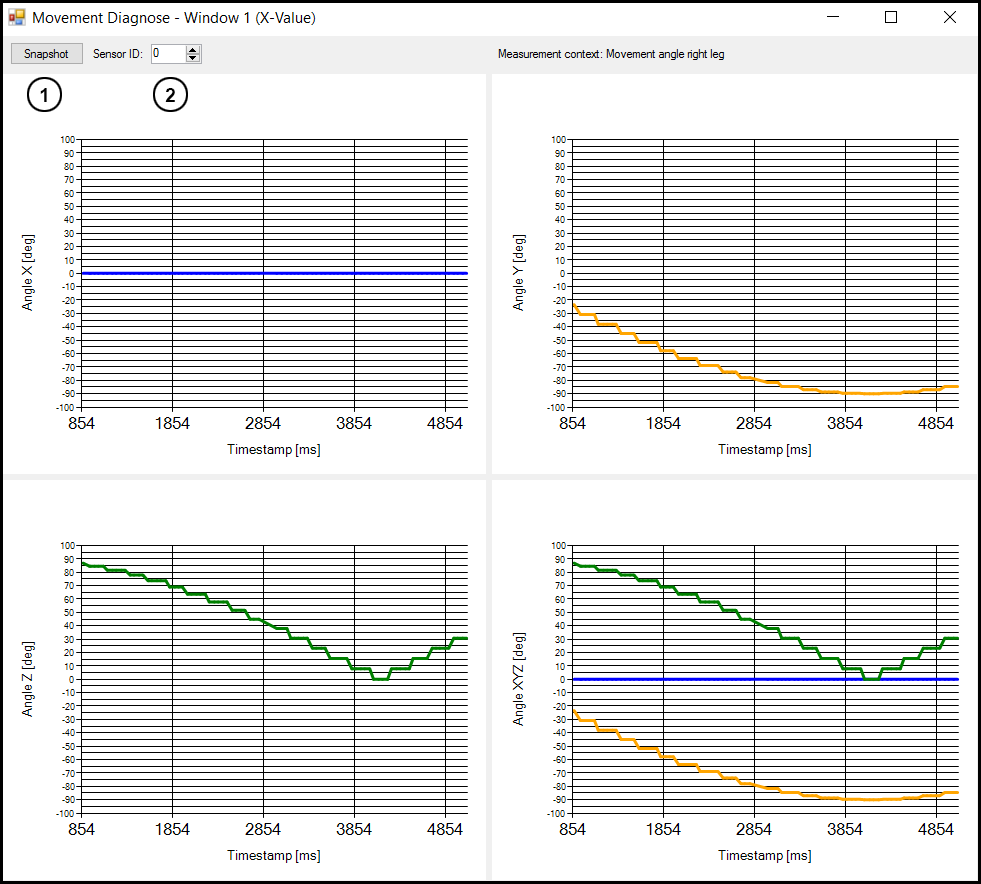
\includegraphics[width=1\linewidth]{03_Grafiken/Messsystem/ClientGraphDiagramm}
\caption[Diagramm Sensorwerte]{Diagramm der Sensorwerte}
\label{fig:clientgraphdiagramm}
\end{figure}




\subsection{Beschreibung HMI - Datenbank}
\label{kap:ClientGraphProgrammDatenbank}
W�hrend des Aufzeichnens von Sensorwerten erfolgt das Abspeichern in eine Datenbank. Diese beinhaltet die Daten f�r jeden Sensor einzeln mit den Beschleunigungswerten in x, y und z, sowie einen Zeitstempel. Die Datenbank kann durch das Bet�tigen des Buttons \textit{Show Database}, in der Hauptansicht des Programms, angezeigt werden (s. Abbildung \ref{fig:clientgraphdatabase}). Durch das Bet�tigen des Up-Down-Selectors erfolgt die Auswahl des entsprechenden Sensors.\\
Bei einer ernueten Messwertaufnahme wird der Datenbankinhalt gel�scht.

\begin{figure}[H]
\centering
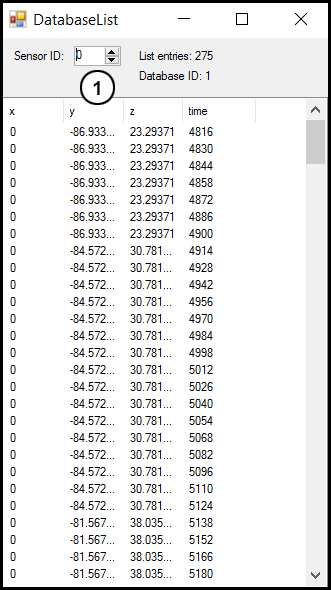
\includegraphics[width=0.5\linewidth]{03_Grafiken/Messsystem/ClientGraphDatabase}
\caption[Datenbank mit Sensorwerten]{Datenbank mit Sensorwerten}
\label{fig:clientgraphdatabase}
\end{figure}

\subsection{Beschreibung Programmaufbau}
\label{kap:ClientGraphCode}
In diesem Kapitel wird zu jeder Funktion (z.B. das Starten einer Messung) die dahinter liegenden Programm-Elemente aufgezeigt und erl�utert. Triviale Funktionalit�ten, wie z.B. das L�schen eines Textfeldes, werden dabei au�er Acht gelassen.

Die Elemente werden dabei mit der in der HMI angegebenen Bezeichnung beschrieben.

\begin{enumerate}
	%
	% Record to db
	%
	\item \textbf{Record to db}\\
	Das Starten einer Messwertaufnahme erfolgt durch das Bet�tigen des Buttons \textit{Record to db}. In der dazugeh�rigen Event-Routine (s. Listing \ref{lst:recordToDb} Zeile 1-19) erfolgt zun�chst eine Abfrage der Button-Beschriftung (Zeile 3), da nur ein Element zum Stoppen / Starten einer Messwertaufnahme genutzt wird. In dieser Abfrage wird ein Dialog eingeblendet, der das L�schen des bisherigen Datenbankinhaltes veranlasst (Zeile 5-9). \\
	Das L�schen der Datenbank erfolgt innerhalb eines Background-Tasks (s. Zeile 23-32). Hierbei wird in Zeile 26 und 27 die Datenbank 1 und 2 mit den entsprechenden Connectionstrings gel�scht. In Zeile 28 und 29 erfolgt das Erstellen der neuen Datens�tze f�r Datenbank 1 und 2. Zeile 30 gibt den Datensatz 1 an die Routine \textit{x\_RunWOrkerCompleted()} weiter. In dieser Routine wird die boolsche Variable \textit{recordIsActive} gesetzt, sodass in der Event-Routine \textit{tcpMsgRecEvent()}, die beim Eintreffen eines Messwerts aufgerufen wird, Werte in die Datenbank geschrieben werden k�nnen. Sobald die Variable wieder zur�ckgesetzt ist, erfolgt kein weiteres Schreiben in die Datenbank.
	\label{lst:recordToDb}
\begin{lstlisting}[language=Java, caption=Messwertaufnahme starten]
private void recordToDb_Click(object sender, EventArgs e)
{
	if (button_recordToDb.Text.Equals("Record to db"))
	{
		if (MessageBox.Show("Delete database content?", "Database re-initialization", MessageBoxButtons.OKCancel, MessageBoxIcon.Question) == DialogResult.OK)
		{
			labelSavedRows.Text = "";
			backgroundWorker_DeleteDb.RunWorkerAsync();
		}
		else ; // Do nothing
	}
	else
	{
		...
		recordIsActive = false;
		savedRowCounter = 0;
		...
	}
}
...
private void backgroundWorker_DeleteDb_DoWork(object sender, DoWorkEventArgs e)
{
	...
	databaseConnection.deleteDatabaseContent(ConnectionString_DB1);
	databaseConnection.deleteDatabaseContent(ConnectionString_DB2);
	dataSet_Db1 = databaseConnection.createDatasetsForDb(ConnectionString_DB1);
	dataSet_Db2 = databaseConnection.createDatasetsForDb(ConnectionString_DB2);
	e.Result = databaseConnection.getTableSizeForDb(dataSet_Db1);
	...
}
...
private void backgroundWorker_DeleteDb_RunWorkerCompleted(object sender, RunWorkerCompletedEventArgs e)
{
	...
	recordIsActive = true;
	maxTableRows_Db1 = (int[])e.Result;
}
\end{lstlisting}
	%
	% Export db to txt
	%
	\item \textbf{Export db to txt file}\\
	Das Exportieren der gespeicherten Messwerte (Formatierung: CSV-Datei, Trennzeichen: Semikolon) erfolgt durch das Bet�tigen des Buttons \textit{Export db to txt}. In der dazugeh�rigen Event-Routine wird dazu ein Background-Task gestartet \ref{lst:exportDb} Zeile 1-16). In dieser Routine wird zun�chst die maximale Zeilenanzahl, sowie die �berschrift f�r das Textdokument gesetzt.\\
	In Zeile 7-15 erfolgt das Schreiben der Daten in eine Textdatei. Diesbez�glich wird f�r jeden Sensor eine seperate Datei mit spezifischen DAteinamen erstellt. Das Setzen des Dateinamens erfolgt im Textfeld \textit{Context} innerhalb der Main-Gui. Wird kein Name angegeben, so tragen die Dateien die Bezeichnung \textit{noname\_x.txt}. \\
	Da w�hrend des Schreibvorgangs alle Buttons deaktiviert werden, erfolgt in der Routine \textit{...RunWorkerCompleted()} das Re-Aktivieren der entsprechenden Elemente.
	\label{lst:exportDb}
\begin{lstlisting}[language=Java, caption=Datenbank exportieren]
private void backgroundWorker_saveDbToTxt_DoWork(object sender, DoWorkEventArgs e)
{
	...
	int[] maxTableRows = databaseConnection.getTableSizeForDb(dataSet_Db1);
	string header = "x[deg];y[deg];z[deg];timestamp[ms]";
	
	for (int i = 0; i < maxTableRows.Length; i++)
	{
		string fileName;
		if (textBox_context.Text != "") fileName = textBox_context.Text + "_" + i + ".txt";
		else fileName = "noname_" + i + ".txt";
		
		using (StreamWriter writer = new StreamWriter(FILE_SAVE_PATH + fileName, false)) writer.WriteLine(header);
		saveDbToFile(i, maxTableRows, fileName);
	}
}
...
private void backgroundWorker_saveDbToTxt_RunWorkerCompleted(object sender, RunWorkerCompletedEventArgs e)
{
	helperFunctions.changeElementEnable(button_exportToTxt, true);
    helperFunctions.changeElementEnable(button_recordToDb, true);
    helperFunctions.changeElementEnable(button_importToDb, true);
}
\end{lstlisting}
	%
	% Import extracted steps
	%
	\item \textbf{Upload steps}\\
	Zun�chst muss in das Textfeld \textit{db name} die Bezeichnung der Tabelle eingegeben werden, in die etwas importiert werden soll (Tabellenname in der externen SQL-Datenbank - s. Beschreibung Kapitel \ref{kap:DatabaseLayout}).
	Durch das Bet�tigen des Buttons erscheint dann ein Dialog, in dem der Bediener eine CSV-Datei (ohne �berschrift) ausw�hlen muss. Diese Textdatei muss folgendes Format des Dateinamens aufweisen: tableX.txt (X steht f�r die Zahl des Sensors, z.B. 0, 1, 2, etc.).\\
	Anschlie�end erfolgt das Hochladen in eine externe SQL-Datenbank.
	In einer sp�teren Version wird es nur noch einen Button geben, mit dem die Schrittfolge automatisch extrahiert und in die externe Datenban k hochgeladen wird.
	\label{lst:uploadSteps}
\begin{lstlisting}[language=Java, caption=Schrittfolge auslagern]
private void button_uploadSteps_Click(object sender, EventArgs e)
{
	...	
	try
	{
		fileId = Int32.Parse(fileName[0]);
		db_name = textBox_dbTableName.Text;
	}
	...
	finally
	{
		if (((fileId >= MIN_TABLE_AMOUNT) && (fileId <= MAX_TABLE_AMOUNT)) && (db_name.Length != 0)) backgroundWorker_loadTxtToDb.RunWorkerAsync();
		else helperFunctions.changeElementText(textBox_Info, "Wrong file id or db name", true);
	}
}
private void backgroundWorker_loadTxtToDb_DoWork(object sender, DoWorkEventArgs e)
{
	...
	xampp_removeContent(db_name, fileId);
	using (StreamReader reader = new StreamReader(directoryTxtImport))
	{
		while (!reader.EndOfStream)
		{
			returnString = reader.ReadLine();
			String[] messageData = returnString.Split(';');
			Decimal[] messageDataAsDecimal = new Decimal[messageData.Length];
			
			for (int j = 0; j < 4; j++) messageDataAsDecimal[j] = Decimal.Parse(messageData[j], CultureInfo.InvariantCulture.NumberFormat);
			if (readCounter > 0) xampp_addContent(db_name, fileId, messageDataAsDecimal);
			...
		}
	}
}
\end{lstlisting}
	%
	% Calibrate Sensors
	%
	\item \textbf{Calibrate Sensors}\\
	Das Starten der Kalibrierung erfolgt durch das Bet�tigen des Buttons \textit{Calibrate Sensors}. In der dazugeh�rigen Event-Routine (s. Listing \ref{lst:calibrateSensor} Zeile 1-9) werden zun�chst die Kalibrierwerte (Zeile 5), sowie der Merker, f�r das Durchf�hren einer Kalibrierung (Zeile 6), zur�ckgesetzt.\\
	In Zeile 8 wird der Button deaktiviert und erst wieder aktiviert wenn die Kalibrierung abgeschlossen ist.\\
	Das Ausf�hren der Kalibrierung erfolgt in der Event-Routine \textit{tcpMsgRecEvent()} (Zeile 11-52), die beim Eintreffen eines Messwerts ausgef�hrt wird. Ist der Button \textit{Calibrate Sensors} deaktiviert und der Merker f�r die durchgef�hrte Kalibrierung \textit{sensorCalibrationSet[]} gesetzt erfolgt das Kalibrieren in den Zeilen 18-36. Dabei wird zu Beginn in den Zeilen 18-20 der Quadrant gepr�ft, in dem sich das \gls{KS} des Sensors befindet. Demnach erfolgt ein Abbruch, wenn ein Sensor sich nicht innerhalb der zul�ssigen Quadranten (s. Abbildung \ref{fig:ZulQuadranten}) befindet.
	
	\begin{figure}[h]
	\centering
	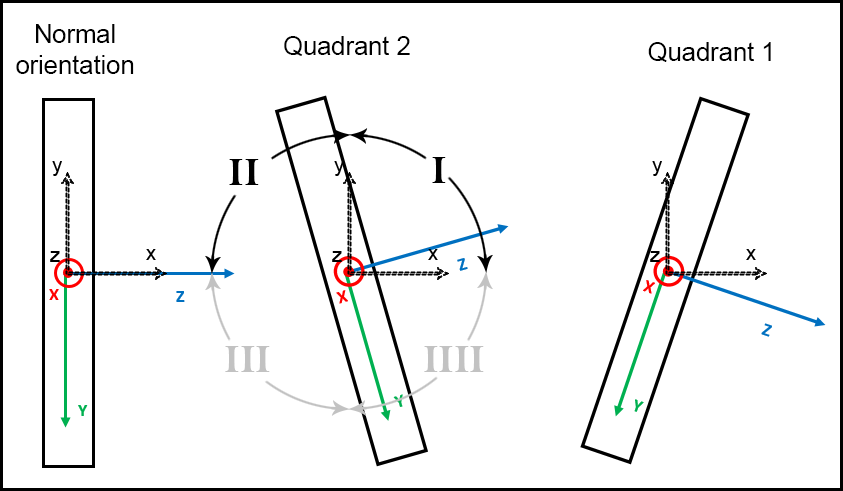
\includegraphics[width=0.7\linewidth]{03_Grafiken/Messsystem/Quadranten}
	\caption[Zul�ssige Quadranten]{Zul�ssige Quadranten}
	\label{fig:ZulQuadranten}
	\end{figure}

	\label{lst:calibrateSensor}
\begin{lstlisting}[language=Java, caption=Sensoren kalibrieren]
private void button_calibrateSensors(object sender, EventArgs e)
{
	for (int i = 0; i < SENSOR_AMOUNT; i++)
	{
		gs_x[i] = 0; gs_y[i] = 0; gs_z[i] = 0;
		sensorCalibrationSet[i] = false;
	}
	buttonCalibrateSensors.Enabled = false;
}
...
private void tcpMsgRecEvent(string[] receivedMessage)
{
	...
	if (sensor_joint_ID <= SENSOR_AMOUNT)
	{
		if ((!sensorCalibrationSet[sensor_joint_ID]) & (!buttonCalibrateSensors.Enabled))
		{
			double alpha = -9999;
			if ((sensorValues[1] >= 0) & (sensorValues[2] < 0)) alpha = -(Math.PI / 2) + Math.Acos((sensorValues[1] * GRAVITATION_EARTH) / GRAVITATION_EARTH);
			else if ((sensorValues[1] >= 0) & (sensorValues[2] > 0)) alpha = (Math.PI / 2) - Math.Acos((sensorValues[1] * GRAVITATION_EARTH) / GRAVITATION_EARTH);
			
			if (alpha != -9999)
			{
				Rx_x[0] = 1;
				Rx_x[1] = 0;
				Rx_x[2] = 0;
				
				Rx_y[0] = 0;
				Rx_y[1] = Math.Cos(alpha);
				Rx_y[2] = -Math.Sin(alpha);
				
				Rx_z[0] = 0;
				Rx_z[1] = Math.Sin(alpha);
				Rx_z[2] = Math.Cos(alpha);

				sensorCalibrationSet[sensor_joint_ID] = true;
				
				for (int i = 0; i < SENSOR_AMOUNT; i++)
				{
					if (!sensorCalibrationSet[i]) break;
					else if (i == SENSOR_AMOUNT - 1) helperFunctions.changeElementEnable(buttonCalibrateSensors, true);
				}			
			}
			else
			{
				helperFunctions.changeElementText(textBox_Info, "Calibration failed!", true);
				helperFunctions.changeElementEnable(buttonCalibrateSensors, true);
			}
		}
	}
	...
}
\end{lstlisting}
	%
	% Show graph
	%
	\item \textbf{Show graph}\\
	Das Visualisieren der Messwerte erfolgt innerhalb eines Hintergrund-Tasks. Diesbez�glich wird der Graph aktualisiert, sobald ein neuer Messwert empfangen wurde. Beim Empfangen eines Messwerts erfolgt der Aufruf der Event-Routine \textit{tcpMsgRecEvent()} (s. Listing \ref{lst:showGraph} Zeile 1-4). Innerhalb dieser Routine wird gepr�ft, ob die Checkbox zum Anzeigen der Visualisierung gesetzt und ob die Windows Form bereits deklariert ist. Ist dies der Fall, so erfolgt die �bergabe aller Messwerte, sowie der Sensor-ID an die Routine \textit{setNewChartData()} (s. Zeile 3).\\
	In dieser Routine wird zun�chst gepr�ft, ob die ausgew�hlte ID (mit dem Up- Down-Selector) mit der �bertragenen Sensor-ID �bereinstimmt. Ist dies der Fall so erfolgt das Setzen eines Events \textit{chartData()} (s. Zeile 8). In der Event-Routine \textit{OnChartEvent()} wird zun�chst gepr�ft, ob die darzustellenden Daten bereits in dem Daten-Array vorhanden sind (Pr�fen gegen Vorinitialisierung -9999). Ist dies der Fall so wird die Routine \textit{setDataToGraph()} aufgerufen (�bergabewert: Sensordaten). In dieser Routine ist das Visualisieren der Messwerte implementiert (s. Zeile 16-24). Dargestellt ist der Code f�r das Setzen der Sensorwerte auf die X-Achse. Zeile 18-19 zeigt das Setzen der Achsbeschriftung und Zeile 21-22 zeigt das Setzen eines Messpunkts.
	\label{lst:showGraph}
\begin{lstlisting}[language=Java, caption=Visualisierung anzeigen]
private void tcpMsgRecEvent(string[] receivedMessage)
{
	if ((checkBox_showGraphs.Checked) && (formCharts != null)) formCharts.setNewChartData(messageDataAsDecimal, sensor_joint_ID);
}

public void setNewChartData(Decimal[] message, int currentSensorID)
{
    if (sensorIdToShow == currentSensorID) this.chartData = message;
}

private void OnChartEvent(object sender, EventArgs e)
{
	if ((chartData[0] != -9999) && (chartData[1] != -9999) && (chartData[2] != -9999) && (chartData[3] != -9999)) setDataToGraph(chartData); dataCounter++;
}

private void setDataToGraph(Decimal[] chartData)
{
	chartX.ChartAreas[0].AxisX.Title = "Timestamp [ms]";
	chartX.ChartAreas[0].AxisY.Title = "Angle " + chartXaxisLabel[0] + " [deg]";	
	...	
	chartSeries[0].Points.AddXY(chartData[3], chartData[0]);
	chartX.Invalidate();
	...	
}
\end{lstlisting}
	%
	% Show database
	%
	\item \textbf{Show database}\\
	Das Darstellen der Datenbank, indem sich die aufgezeichneten Messwerte befinden, erfolgt durch das Setzen der entsprechenden Checkbox. Das Pr�fen, ob die Checkbox gesetzt ist erfolgt inerhalb der verbundenen Event-Routine (s. Listing \ref{lst:showDb} Zeile 4). Entsprechend der Datenbank-ID wird die Datenbank ausgew�hlt und eine Liste mit dessen Inhalt erzeugt (s. Zeile 6) und dargestellt (s. Zeile 7).
	\label{lst:showDb}
\begin{lstlisting}[language=Java, caption=Datenbank anzeigen]
private void checkBox_showDatabase_CheckedChanged(object sender, EventArgs e)
{
	...
	if (((CheckBox)sender).Checked)
	{
		dataBaseList = new DatabaseList(this, dataSet_Db1, databaseConnection, databaseId);
		dataBaseList.Show();
	}
	else try dataBaseList.Close();
	...
}
\end{lstlisting}
\end{enumerate}

